\documentclass{IEEEtran}
\usepackage{cite}
\usepackage{amsmath,amssymb,amsfonts}
\usepackage{algorithmic}
\usepackage{graphicx}
\usepackage{pgfplots}
\usepackage{tikz}
\usepackage{textcomp}
\usepackage{booktabs}
\usepackage{listings}
\usepackage{xcolor} % for setting colors
\definecolor{vblue}{RGB}{49,49,255}
\definecolor{vgreen}{RGB}{104,180,104}

\usepackage {tikz}
\usetikzlibrary {positioning}
%\usepackage {xcolor}
\definecolor {processblue}{cmyk}{0.96,0,0,0}

\definecolor{light-gray}{gray}{0.95} %the shade of grey that stack exchange uses
% set the default code style
\lstset{
	basicstyle=\ttfamily,  
	backgroundcolor=\color{light-gray}
}
 \lstdefinestyle{cpp}{
 	language=C++,
 	basicstyle=\small\ttfamily,
 	keywordstyle=\color{vblue},
 	identifierstyle=\color{black},
 	commentstyle=\color{vgreen},
 	numberstyle=\tiny\color{black},
 	numbersep=10pt,
 	tabsize=4,
 	moredelim=*[s][\colorIndex]{[}{]},
 	literate=*{:}{:}1
 }

\def\BibTeX{{\rm B\kern-.05em{\sc i\kern-.025em b}\kern-.08em
		T\kern-.1667em\lower.7ex\hbox{E}\kern-.125emX}}
\begin{document}
\title{Parallel Congruence Closure SAT solver}
\author{Enrico Martini, VR445204}
\maketitle
\begin{abstract}
 In this report is presented a parallel implementation of a congruence closure algorithm for deduction in ground equational theories, able to solve a set of clauses in the quantifiers free fragment of first order logic, based on equality among variables, constants, function applications, recursive data structures with their elements and elements of arrays.
\end{abstract}
\section{Introduction}
The first theory considered is the class of SMT problems is called EUF (Equality with Uninterpreted Functions), containing atoms that are equalities between terms built over uninterpreted function symbols. EUF (i.e., SAT modulo the theory of congruences) is important in applications such as the verification of pipelined processors, where, if the control is verified, the concrete data operations can be abstracted by uninterpreted function symbols.\cite{NIEUWENHUIS2007557} It is the most important theory because its congruence closure algorithm is the core of the entire solver. The implemented algorithm also integrates the theory of lists $\mathcal{T}_{cons}$ and the theory of array without extensionality $\mathcal{T}_A$. In order to reduce the computational complexity of the alghoritm, a parallel version of the solver has been implemented.
\section{Methodology}
\subsection{Algorithm}
The most interesting feature of this implementation is the organization of the information within the data structures, shaped to be efficient.
\paragraph{Node} 
The design of the \verb|Node| structure was mainly inspired by the interpretation of  \textit{'The Calculus of Computation'}\cite{10.5555/1324777}, which describes a resolution procedure for the above mentioned theories. The \verb|id| field holds the node’s unique identification number; the \verb|fn| field holds the constant or function symbol and the \verb|args| field holds a list of identification numbers representing the function arguments. The \verb|find| field holds the identification number of another node (possibly itself) in its congruence class. Following a chain of \verb|find| references leads to the representative of the congruence class. A representative node’s find field points to the node itself. If a node is the representative for its congruence class, then its \verb|ccpar| (for congruence closure parents) field stores the set of all parents of all nodes in its congruence class.
\begin{lstlisting}[style=cpp]
class Node{
private:
	std::string 		fn;                  
	int			 		id;                
	std::vector<int> 	args; 
	int			 		find;              
	std::vector<int>	ccpar;
};
\end{lstlisting}
\paragraph{Clause} 
The \verb|Clause| class is used to save nodes while maintaining the given input relationship. It allows two nodes to be related but has no methods to compare them, as they are used in another class.
\begin{lstlisting}[style=cpp]
class Clause{
private:
	Node n1;
	Node n2;
	bool is_equal;
}
\end{lstlisting}
\paragraph{Formula}
The \verb|Formula| class contains a single vector of clauses. This structure is the exact transposition of the given input string to be resolved. Once the formula is created the initial string can be discarded because all relevant information has been saved.
\begin{lstlisting}[style=cpp]
class Formula{
private:
	std::vector<Clause> v_set;
};
\end{lstlisting}
\paragraph{Sat}
The \verb|Sat| class acts as a wrapper for the entire library. It contains methods for interfacing with the solver and methods for string parsing. Inside it is saved the initial translated formula and the set of nodes on which the congruence closure will be performed. There are also two index vectors, useful for checking the type of elements. In this case, since the array theory is also included, it has been mandatory to introduce a type checking system that is able to detect any errors in the provided string, such as the comparison between two arrays that is not possible to do in the array theory without extensionality, due to the fact that the decision procedure for T$_A$-satisfiability of quantifier-free $\sum_A$-formula $\mathcal{F}$ is based on a reduction to T$_E$-satisfiability via applications of the \textit{(read-over-write)} axioms \cite{10.5555/1324777}, shown in equations \ref{read-over-write} and \ref{read-over-write2}.

\begin{align}
	\label{read-over-write}
	&\forall a,v,i,j. i = j \to select(store(a,i,e),j) = e \\
	\label{read-over-write2}
	&\forall a,v,i,j. i \ne j \to select(store(a,i,e),j) = select(a,j)
\end{align}

There are two functions to check that the string is acceptable to the parser and then to the solver. While the \verb|is_legal| function checks that an array type element is not in an equal relationship, the \verb|well_formed| function checks that the syntax accepted as input is valid, for example by checking the number of open and closed brackets. The \verb|transform_node|, \verb|initialize_DAG|, \verb|split| and \verb|split_arguments| functions are used to populate the node vector and reconstruct the formula, preparing the necessary for resolution. The \verb|classic_congruence_closure| function performs the congruence closure by calling the functions \verb|FIND|, \verb|UNION|, \verb|CCPAR|, \verb|CONGRUENT| and \verb|MERGE|. These methods are a realization of the algorithm explained in chapter 9 of the Bradley-Manna book \cite{10.5555/1324777}, which consists of calling the recursive function \verb|MERGE| for each equation in order to build the congruence classes. Once the equalities are completed, it is checked that for each inequality the two elements that must be different are not in the same class of equivalence. The \verb|list_congruence_closure| function makes strings that also belong to list theory acceptable to the solver. After initializing the DAG, for each node $n$ such that \verb|n.fn| $=$ \textit{'cons'}, it adds \verb|car(n)| to the DAG and merge \verb|car(n)| with \verb|n.args[1]| and \verb|cdr(n)| to the DAG and merge \verb|cdr(n)| with \verb|n.args[2]|. After doing this pre-processing operation, the \verb|classic_congruence_closure| is performed. If the procedure fails, then the formula is unsatisfable, but if the procedure is successful, there is another check to see if there are both atoms and lists in the same congruence class. In that case the formula will be unsatisfable by axiom \textit{(atom)} shown in equation \ref{atom}, otherwise satisfable.
\begin{equation}
	\label{atom}
	\forall x,y. \neg atom(cons(x,y))
\end{equation}
The \verb|detect_store| function is executed before parsing the formula. According to the axioms, for each \verb|select(store(a,i,e),j)| two formulas are created, one in case \verb|i| is equal to \verb|j| and one in case \verb|i| is different from \verb|j|. The recursive \verb|solve| function after checking that the string is properly formatted, if the string does not contain the $store$ keyword, the congruence closure is performed, while if the $store$ keyword is detected, \verb|solve| is called on the formulas generated by \verb|detect_store|. The \verb|SOLVE| function solves a formula in disjunctive normal form. A formula is in disjunctive normal form (DNF) if it is a disjunction of conjunctions of literals. The function divides the formula into a vector of disjointed conjunctions. Once the strings have been prepared, they are divided into batches of variable size depending on the processor on which the solver is running. Each core the processor is equipped with takes charge of a batch, going to call the \verb|solve| function in parallel. If only one of these formulas is satisfable, the procedure ends.
\begin{lstlisting}[style=cpp]
class Sat{
private:
	Formula 			f;
	std::vector<Node> 	n_set;
	std::vector<int> 	atoms;
	std::vector<int> 	arrays;

	bool	is_legal();
	bool 	well_formed(std::string s);
	
	int 	transform_node(std::string n);
	void 	initialize_DAG(std::string input);
	std::vector<std::string> 
			split(std::string s);
	std::vector<std::string> 
			split_arguments(std::string s);

	int 			 FIND(int index);
	void 			 UNION(int i1, int i2);
	std::vector<int> CCPAR(int index);
	bool 			 CONGRUENT(int i1, int i2);
	void 			 MERGE(int i1, int i2);

	bool 	classic_congruence_closure();
	bool 	list_congruence_closure();
	
public:
	static std::vector<std::string> 
			detect_store(std::string input);
	static bool solve(std::string s);
	static bool 
	SOLVE(std::string input,std::string mode);
};
\end{lstlisting}
Finally, a heuristic was introduced trying to achieve further improvements in performance. After initializing the DAG, a forbidden list is created in which all the inequality clauses are present. Before performing the congruence closure, it is checked if equality and inequality with the same nodes are present. In this way it is possible to decide that the formula is unsatisfactory without even performing the congruence closure. In case the procedure starts, at each merge it is checked if the elements to be merged are part of the list of clauses contained in the forbidden list. If so, the procedure ends before it is even finished.

\subsection{Equality theory congruence closure example}
Let's see now with a practical example how congruence closure is performed.
The formula \ref{example} is passed as an argument to the \verb|solve| function. 
\begin{equation}
	\label{example}
	\mathcal{F} : x = y \land f(x) \ne f(y)
\end{equation}
\begin{lstlisting}
x=y&f(x)!=f(y)
\end{lstlisting}
The string is well formatted and contains no \textit{store} keyword, so the parser creates four nodes: two constants ($x$ and $y$) and two functions ($f(x)$ and $f(y)$). At this point there are four congruence classes, one for each element. Every element is therefore representative of its own class.
\begin {center}
\resizebox{3.5cm}{!}{
\begin {tikzpicture}[-latex ,auto ,node distance =2 cm and 2cm ,on grid ,
semithick ,
state/.style ={ circle ,top color =white , bottom color = white ,
	draw,black , text=black , minimum width =0.5 cm}]
\node[state] (N0) {0 : x};
\node[state] (N1) [right=of N0]{1 : y};
\node[state] (N2) [above =of N0]{2 : f};
\node[state] (N3) [above right=of N0] {3 : f};
\path (N2) edge [above] node[left] {} (N0);
\path (N3) edge [above] node[left] {} (N1);
\end{tikzpicture}
}
\end{center}

\begin{lstlisting}
node		find		ccpar
________________________________________
0x		0		2
1y		1		3
2f->0		2		-
3f->1		3		-
\end{lstlisting}

Initially, the $x=y$ clause is taken into account. The \verb|merge| between $x$ and $y$ is made. 
\begin{lstlisting}
MERGE 0 1
UNION 0 1
\end{lstlisting}
Now $x$ and $y$ are part of the same congruence class and the class representative is $x$. The \verb|ccpar| of $y$ have been moved to $x$, which now contains all the useful information for the congruence class.
\begin {center}
\resizebox{3.5cm}{!}{
	\begin {tikzpicture}[-latex ,auto ,node distance =2 cm and 2cm ,on grid ,
	semithick ,
	state/.style ={ circle ,top color =white , bottom color = white ,
		draw,black , text=black , minimum width =0.5 cm}]
	\node[state] (N0) {0 : x};
	\node[state] (N1) [right=of N0]{1 : y};
	\node[state] (N2) [above =of N0]{2 : f};
	\node[state] (N3) [above right=of N0] {3 : f};
	\path (N2) edge [above] node[left] {} (N0);
	\path (N3) edge [above] node[left] {} (N0);
	\path (N0) edge[,-,densely dotted] [above] node[left] {} (N1);
\end{tikzpicture}
}
\end{center}

\begin{lstlisting}
node		find		ccpar
________________________________________
0x		0		23
1y		0		-
2f->0		2		-
3f->1		3		-
\end{lstlisting}

Indeed, the \verb|merge| is recursively done between $f(x)$ and $f(y)$, since they are parents of $x$ and $y$, have the same name, the same number of arguments and the arguments belong to the same congruence class.
\begin{lstlisting}
MERGE 2 3 ?
CONGRUENT 2 3 = 1
MERGE 2 3
UNION 2 3
\end{lstlisting}

\begin {center}
\resizebox{3.5cm}{!}{
	\begin {tikzpicture}[-latex ,auto ,node distance =2 cm and 2cm ,on grid ,
	semithick ,
	state/.style ={ circle ,top color =white , bottom color = white ,
		draw,black , text=black , minimum width =0.5 cm}]
	\node[state] (N0) {0 : x};
	\node[state] (N1) [right=of N0]{1 : y};
	\node[state] (N2) [blue,above =of N0]{2 : f};
	\node[state] (N3) [blue,above right=of N0] {3 : f};
	\path (N2) edge [above] node[left] {} (N0);
	\path (N3) edge [above] node[left] {} (N0);
	\path (N0) edge[,-,densely dotted] [above] node[left] {} (N1);		\path (N2) edge[,blue,-,densely dotted] [above] node[left] {} (N3);
\end{tikzpicture}
}
\end{center}

\begin{lstlisting}
node		find		ccpar
________________________________________
0x		0		23
1y		0		-
2f->0		2		-
3f->1		2		-
\end{lstlisting}

At this point the equalities are solved. We begin to see for each inequality if its elements belong to the same congruence class. In this case $f(x)!=f(y)$, but from the last merge it can be seen that $f(x)$ and $f(y)$ belong to the same congruence class, so the formula is unsatisfable. 

\begin {center}
\resizebox{3.5cm}{!}{
	\begin {tikzpicture}[-latex ,auto ,node distance =2 cm and 2cm ,on grid ,
	semithick ,
	state/.style ={ circle ,top color =white , bottom color = white ,
		draw,black , text=black , minimum width =0.5 cm}]
	\node[state] (N0) {0 : x};
	\node[state] (N1) [right=of N0]{1 : y};
	\node[state] (N2) [blue,above =of N0]{2 : f};
	\node[state] (N3) [blue,above right=of N0] {3 : f};
	\path (N2) edge [above] node[left] {} (N0);
	\path (N3) edge [above] node[left] {} (N0);
	\path (N0) edge[,-,densely dotted] [above] node[left] {} (N1);		\path (N2) edge[,-,red] [above] node[left] {} (N3);
\end{tikzpicture}
}
\end{center}

\begin{lstlisting}
UNSAT
\end{lstlisting}

\section{Validation}


\section{Benchmarks}
\begin{table}[htpb]
	\centering
	\caption{Performance results with use of forbidden list}
	\label{tab:fl}
	\resizebox{\columnwidth}{!}{%
		\begin{tabular}{|c|l|l|r|r|r|}
			\hline
			\textbf{Test} & \textbf{\#Formulas} & \textbf{\#Equations} & \textbf{Sequential (s)} & \textbf{Parallel (s)} & \textbf{Speedup} \\ \hline
			      7       & 128                 & 1920                 &                  0,0128 &                0,0001 &             97,3 \\ \hline
			      8       & 256                 & 4352                 &                  0,0273 &                0,0003 &            107,6 \\ \hline
			      9       & 512                 & 9728                 &                  0,0605 &                0,0007 &             88,6 \\ \hline
			     10       & 1024                & 21504                &                  0,1341 &                0,0024 &             57,0 \\ \hline
			     11       & 2048                & 47104                &                  0,2964 &                0,0099 &             29,9 \\ \hline
			     12       & 4096                & 102400               &                  0,6639 &                0,0430 &             15,5 \\ \hline
			     13       & 8192                & 221184               &                  1,5309 &                0,1854 &              8,3 \\ \hline
			     14       & 16384               & 475136               &                  3,7426 &                1,7264 &              2,2 \\ \hline
			     15       & 32768               & 1015808              &                 13,8145 &                9,4844 &              1,5 \\ \hline
		\end{tabular}%
	}
\end{table}

\section{Performance Analysis}



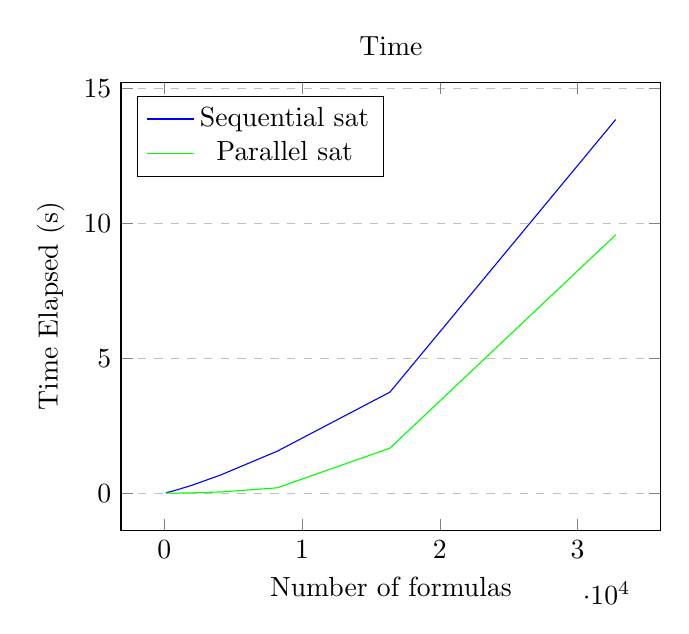
\begin{tikzpicture}
\begin{axis}[
title={Time},
ylabel={Time Elapsed (s)},
xlabel={Number of formulas},
legend pos=north west,
ymajorgrids=true,
grid style=dashed,
]

\addplot[color=blue]
coordinates {
	(128,0.0117)(256,0.0290)(512,0.0612)(1024,0.1374)(2048,0.2988)(4096,0.6736)(8192,1.5526)(16384,3.7465)(32768,13.8530)
};
\addplot[color=green]
coordinates {
	(128,0.0001)(256,0.0003)(512,0.0008)(1024,0.0026)(2048,0.0103)(4096,0.0442)(8192,0.1968)(16384,1.6690)(32768,9.5786)
};

\legend{Sequential sat,Parallel sat}

\end{axis}
\end{tikzpicture}

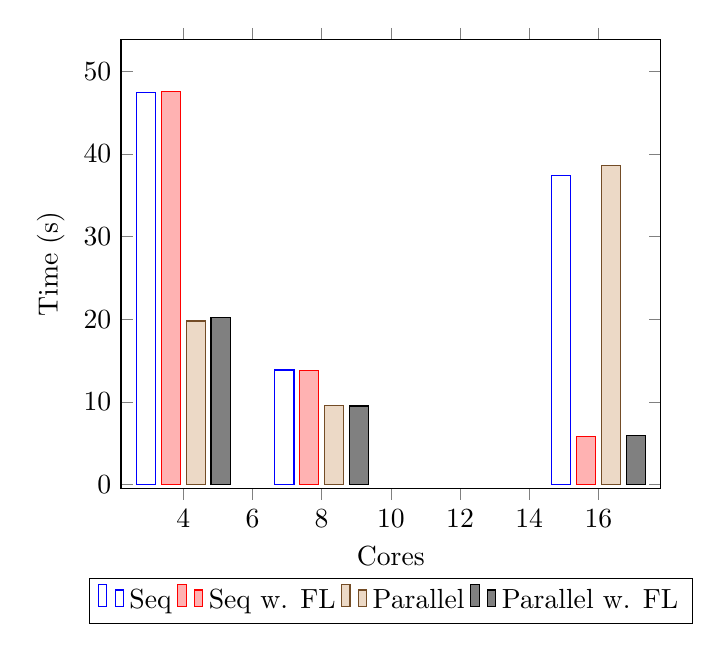
\begin{tikzpicture}
\begin{axis}[
x tick label style={
	/pgf/number format/1000 sep=},
ylabel=Time (s),
enlargelimits=0.15,
legend style={at={(0.5,-0.2)},
	anchor=north,legend columns=-1},
ybar,
bar width=7pt,
xlabel=Cores\\
]
\addplot[color=blue,domain=15:15]
coordinates {(4,47.4944)(8,13.8530)(16,37.3613)};
\addplot 
coordinates {(4,47.5747)(8,13.8145)(16,5.8145)};
\addplot 
coordinates {(4,19.7812)(8,9.5786)(16,38.5786)};
\addplot 
coordinates {(4,20.1922)(8,9.4844)(16,5.9145)};
\legend{Seq,Seq w. FL ,Parallel, Parallel w. FL}
\end{axis}
\end{tikzpicture}


\section{Conclusion}

\bibliography{biblio}
\bibliographystyle{ieeetr}


\appendix
% Please add the following required packages to your document preamble:
% \usepackage{booktabs}
% \usepackage{graphicx}
\begin{table}[htpb]
	\centering
	\caption{}
	\label{tab:my-table}
	\resizebox{\textwidth}{!}{%
		\begin{tabular}{@{}cclc@{}}
			\toprule
			\textbf{Theory} & \textbf{Source}   & \textbf{Formula}                                                                                           & \textbf{Result} \\ \midrule
			Equality        & Bradley-Manna     & f(x)=f(y)\&x!=y                                                                                            & SAT             \\
			&                   & x=y\&f(x)!=f(y)                                                                                            & UNSAT           \\
			&                   & f(a,b)=a\&f(f(a,b),b)!=a                                                                                   & UNSAT           \\
			&                   & f(f(f(a)))=a\&f(f(f(f(f(a)))))=a\&f(a)!=a                                                                  & UNSAT           \\
			&                   & f(f(f(a)))=f(f(a))\&f(f(f(f(a))))=a\&f(a)!=a                                                               & UNSAT           \\
			&                   & f(x,y)=f(y,x)\&f(a,y)!=f(y,a)                                                                              & SAT             \\
			&                   & f(g(x))=g(f(x))\&f(g(f(y)))=x\&f(y)=x\&g(f(x))!=x                                                          & UNSAT           \\
			& IC Tests          & b=d\&f(b)=d\&f(d)=a\&a!=b                                                                                  & UNSAT           \\
			&                   & a=b1\&b1=b2\&b2=b3\&b3=c\&f(a1,a1)=a\&f(c1,c1)=c\&a1=c1\&a!=c                                              & UNSAT           \\
			& Z3 Benchmark      & f1!=f2\&f3(f4,f5,f6,f7,f8(f9))!=f1\&f3(f4,f5,f6,f7,f10)=f1\&f10=f8(f9)\&f10=f8(f9)\&f3(f4,f5,f6,f7,f10)=f1 & UNSAT           \\
			&                   & f1!=f2\&f3(f4,f5,f6,f7,f8(f9))!=f1\&f3(f4,f5,f6,f7,f10)=f1\&f10=f8(f9)\&f3(f4,f5,f6,f7,f10)=f1             & UNSAT           \\
			&                   & f1!=f2\&f3(f4,f5,f6,f7,f8(f9))!=f1\&f3(f4,f5,f6,f7,f10)=f1\&f10=f8(f9)                                     & UNSAT           \\
			List            & Bradley Manna     & x1=x2\&y1=y2\&cons(x1,y1)!=cons(x2,y2)                                                                     & UNSAT           \\
			&                   & x=y\&car(x)!=car(y)                                                                                        & UNSAT           \\
			&                   & x=y\&cdr(x)!=cdr(y)                                                                                        & UNSAT           \\
			&                   & car(cons(x,y))!=x                                                                                          & UNSAT           \\
			&                   & cdr(cons(x,y))!=y                                                                                          & UNSAT           \\
			&                   & !atom(cons(x,y))                                                                                           & SAT             \\
			&                   & atom(x)\&cons(car(x),cdr(x))=x                                                                             & UNSAT           \\
			&                   & car(x)=car(y)\&cdr(x)=cdr(y)\&f(x)!=f(y)\&!atom(x)\&!atom(y)                                               & UNSAT           \\
			&                   & car(x)=y\&cdr(x)=z\&x!=cons(y,z)                                                                           & SAT             \\
			& Intermediate exam & f(b)=b\&f(f(b))!=car(cdr(cons(f(b),cons(b,d))))                                                            & UNSAT           \\
			Array           & Bradley-Manna     & i=k\&select(store(x,i,v),k)!=v                                                                             & UNSAT           \\
			&                   & i!=k\&select(store(x,i,v),k)!=select(x,k)                                                                  & UNSAT           \\
			&                   & i1=j\&i1!=i2\&select(a,j)=v1\&select(store(store(a,i1,v1),i2,v2),j)!=select(a,j)                           & UNSAT           \\
			& Intermediate exam & e=select(store(a,i,e),j)\&select(a,j)!=e                                                                   & SAT             \\ \bottomrule
		\end{tabular}%
	}
\end{table}
















\end{document}